In base al tipo di radiazione può cambiare il meccanismo di interazione con la materia. Vedremo quindi i diversi meccanismi con cui le radiazioni interagiscono con la materia, con conseguente perdita di energia. Cercheremo dunque di stimare anche la perdita di energia delle particelle nella materia, cioè di trovare espressioni quantitative che ci permettano di capire quali sono i parametri che influenzano la perdita di energia.

Tale argomento ci interessa perché lo studio dei diversi rivelatori di particelle si basa sui meccanismi di interazione, che usano per misurare le particelle.

Concentriamoci innanzitutto sulle particelle cariche pesanti, cioè dal protone in su. In realtà in questa categoria rientrano anche le particelle di massa intermedia (muoni, pioni), aventi massa minore di quella del protone ma non piccola quanto quella dell'elettrone, per cui hanno un comportamento maggiormente simile a quello delle particelle pesanti.

\section{Principali meccanismi}

Vediamo adesso quali sono i meccanismi con cui le particelle pesanti interagiscono con la materia.

\subsection{Interazione coulombiana (inelastica) con gli elettroni atomici}

\E la modalità con cui le particelle perdono maggiormente energia all'interno della materia.

Cerchiamo di quantificare il numero di interazioni con gli elettroni che avvengono durante il tragitto delle particelle all'interno della materia. Vediamo allora quanta energia può essere trasferita al massimo in una singola collisione: se $E$ è l'energia iniziale, al massimo in un urto si perde un'energia pari a
\begin{equation*}
    E_{\rm urto}^{\rm max}=4E\frac{m_e}{m}
\end{equation*}
dove $m_e$ è la massa dell'elettrone e $m$ la massa della particella incidente. Ne segue che maggiore è la massa della particella, minore sarà l'energia che può essere trasferita in una singola collisione.

Facciamo un esempio: se la particella incidente è un protone, allora l'energia massima trasferita in una collisione sarà
\begin{equation*}
    E_{\rm urto}^{\rm max}
    =4E\frac{m_e}{m_p}
    \sim \frac{1}{500} E
\end{equation*}
%Se sostituiamo diventa, con M massa della particella in rapporto alla massa del protone. Se la particella incidente è un protone, allora $M=1$ è un singolo urto viene trasferita al massimo $1/500$ dell'energia iniziale. 
Ne segue che se ad ogni urto venisse ceduta la quantità massima di energia, ci vorrebbero 500 collisioni perché si perda tutta l'energia a disposizione. Nella realtà le collisioni sono di più perché abbiamo usato un valore massimo, ma nei fatti avvengono anche trasferimenti di energia minore.

Da tale relazione capiamo che una particella carica pesante, quando attraversa la materia, subisce diverse collisioni con gli elettroni atomici e in ognuna di queste perde una piccola parte della sua energia; pertanto l'energia diminuisce gradualmente, a piccoli passi, fatto che ha un effetto su quello che si misura e sul percorso che può effettuare la particella.

Il risultato del passaggio di una particella all'interno della materia è che, cedendo energia ad ogni collisione agli elettroni atomici, questi ultimi, ricevendo energia, si eccitano oppure possono addirittura, se l'energia è sufficiente, essere strappati dall'atomo, sfuggendo al legame atomico; in quest'ultimo caso può avvenire un processo di ionizzazione. Talvolta gli elettroni che vengono strappati possono produrre delle ionizzazioni secondarie, perché possiedono energie elevate. Se ciò avviene, questi elettroni prendono il nome di \textit{raggi} $\delta$.

Riassumendo: una particella carica pesante, attraversando un materiale, perde energia attraverso multiple collisioni con gli elettroni atomici, i quali possono eccitarsi o addirittura essere strappati dall'atomo e di conseguenza nel tragitto seguito dalla particella si vengono a creare atomi eccitati o addirittura ioni, e la velocità (quindi l'energia) della particella gradualmente diminuirà fino a che questa non si arresta del tutto.

\subsection{Interazione (elastica) con i nuclei}

Può anche avvenire un'interazione elastica con i nuclei che compongono il materiale. Questo processo è meno importante, perciò l'energia persa con tale fenomeno, rispetto a quella persa per interazione coulombiana, è trascurabile. Per capirne il motivo basta pensare alla sezione d'urto, ossia alla probabilità che avvenga un evento di questo tipo: dobbiamo confrontare le dimensioni di un atomo con quelle di un nucleo, per cui c'è un fattore $10^5$ tra le due sezioni d'urto.

Tale interazione diventa importante quando le dimensioni della particella incidente sono simili a quelle del nucleo che compongono il materiale (ad esempio particelle $\alpha$ che incidono su idrogeno), ma di solito si trascura.

\subsubsection{Altri meccanismi}
Avvengono poi altri meccanismi ancora meno rilevanti.

\begin{itemize}
    \item Può verificarsi emissione di radiazioni di frenamento (bremsstrahlung), il quale è un meccanismo più importante per le particelle leggere, mentre per quelle pesanti è trascurabile in quanto la sezione d'urto per bremsstrahlung dipende all'inverso del quadrato della massa della particella incidente.
    \item Può avvenire l'emissione di luce Cherenkov, cioè emissione di luce perché la particella ha velocità superiore alla velocità della luce nel mezzo attraversato. Anche questo contributo è trascurabile rispetto all'interazione coulombiana.
    \item Possono avvenire processi di interazione nucleare.
\end{itemize}

\section{Relazione di Bethe-Bloch}
Abbiamo visto che se ci concentriamo sulle particelle cariche pesanti dobbiamo semplicemente andare a valutare quanta energia viene persa attraverso l'interazione coulombiana con gli elettroni atomici. Siamo allora interessati a calcolare l'energia persa per unità di percorso, dunque vogliamo conoscere qual è l'energia $\dd{E}$ che perde la particella dopo aver percorso uno spazio infinitesimo $\dd{x}$ a seguito dei meccanismi sopracitati.

In altre parole, siamo interessati a calcolare lo \textbf{Stopping Power} o \textit{perdita di energia specifica}, che si indica con $\dv*{E}{x}$. Essa si esprime in $\rm MeV/cm$.\footnote{Il motivo per cui si usano i centimetri anziché i metri è che le particelle cariche pesanti percorrono lunghezze piccole.}

Il problema dello stopping power fu affrontato per primo da Bohr, producendo una teoria che si basava su argomenti classici. Tale teoria fu successivamente ripresa da Bethe e Bloch i quali, usando la meccanica quantistica, giunsero alla formula di Bethe-Bloch\footnote{Di questa esistono diverse formulazioni. Noi faremo riferimento a quella del Particle Data Group. \url{https://pdg.lbl.gov/2022/reviews/rpp2022-rev-passage-particles-matter.pdf}}:

\begin{equation*}
    \expval{-\dv{E}{x}}
    =Kz^2\frac{Z}{A} \frac{1}{\beta^2} \qty[ \frac{1}{2}\ln{\frac{2m_e c^2 \beta^2 \gamma^2 W_{\rm max}}{I^2}} - \beta^2 - \frac{\delta(\beta \gamma)}{2} ]
\end{equation*}

Tale formula descrive la perdita di energia media per unità di percorso. Rispetto a prima aggiungiamo il termine "media" perché la perdita di energia non è sempre la stessa per questioni di fluttuazioni statistiche. Inoltre il segno meno indica il fatto che è una perdita di energia, cioè $\dd{E}$ deve essere negativo perché l'energia sta diminuendo.

\begin{minipage}{0.295\textwidth}
    \begin{figure}[H]
        \centering
        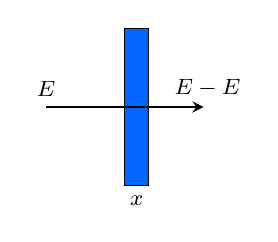
\begin{tikzpicture}
            \draw[fill=blue!60!cyan!] (0,-1) rectangle (+0.3cm,+1cm);
            \node[below] at (0.15,-1) {\footnotesize$\dd{x}$};
            \draw[thick, -stealth] (-1,0) node [above] {\footnotesize$E$} -- (1,0) node [above right] {\footnotesize\hspace{-0.5cm}$E - \dd{E}$};
        \end{tikzpicture}
    \end{figure}
\end{minipage}
\begin{minipage}{0.7\textwidth}
    \vspace{0.35cm}In questa formula stiamo supponendo di avere delle particelle cariche pesanti incidenti, con un'energia $E$, che devono attraversare uno spessore infinitesimo $\dd{x}$ di materiale. Una volta attraversato questo spessore sarà stata persa una parte dell'energia, quindi la particella avrà energia residua $E - \dd{E}$.
\end{minipage}

\vspace{0.3cm}La relazione di Bethe-Bloch ci dice che in media la variazione $\dv*{E}{x}$ dipende da:

\begin{itemize}
    \item Una costante $K=4 \pi N_A r_e^2 m_e c^2=0.307 \; \rm MeV \, mol^{-1} \, cm^2$;
    \item Il quadrato della carica della particella incidente, indicata con $z^2$. Tale dipendenza ci permette di identificare la particella incidente: infatti, se ad esempio confrontiamo un protone con una particella $\alpha$, a parità di energia incidente, essendo una relazione quadratica, il protone perde un quarto di energia di quella persa dall'$\alpha$;
    \item $1/\beta^2$, dove $\beta$ è definito come il rapporto della velocità della particella rispetto alla velocità della luce nel vuoto ($\beta=v/c$). Da un punto di vista classico $\beta^2$ è proporzionale all'energia, in quanto
    \begin{equation*}
        E_k
        =\frac{1}{2}mv^2
        =\frac{1}{2}m \beta^2 c^2
        \implies
        \frac{1}{\beta^2} \propto \frac{1}{E}
    \end{equation*}
    Tale dipendenza ci dice che se la particella incidente ha bassa energia, ci aspettiamo un'alta perdita di energia, perché l'andamento è iperbolico ($1/E$);
    \item Il rapporto $Z/A$, cioè numero atomico/numero di massa del mezzo. Esso vale $0,5$ per i nuclei più leggeri, ma man mano che il nucleo diventa pesante il numero di neutroni diventa maggiore di quello dei protoni, per cui $Z/A$ risulterà minore di $0,5$. Deduciamo che le particelle perdono maggiormente energia se incidono su materiali leggeri.
\end{itemize}

Le prime tre sono dipendenze dalle caratteristiche della particella incidente, l'ultima dalle proprietà del mezzo.

Passiamo adesso ad analizzare i termini tra parentesi.

Il primo termine prende il nome di \textit{risalita relativistica}, il quale ha l'andamento di $\ln E$ (in quanto compare il termine $\beta^2 \propto E$). Figurano poi altri fattori quali

\begin{itemize}[label=$-$]
    \item il fattore di Lorentz $\gamma$, definito come $\gamma=\frac{1}{\sqrt{1 - \beta^2}}$;
    \item $W_{\rm max}$, che rappresenta la perdita di energia massima in una singola collisione;
    \item il potenziale di ionizzazione medio $I$, ossia l'energia che in media è necessaria per la ionizzazione. Esso è un valore medio perché quando forniamo energia ad un atomo a volte produciamo ionizzazione mentre altre volte l'energia viene persa per eccitazione, quindi tale energia sarà più alta del lavoro di estrazione di un elettrone perché una parte viene persa per eccitazione degli atomi.
\end{itemize}

Abbiamo poi un termine correttivo $\delta$, detto \textit{correzione di densità}: esso si inserisce perché il campo elettrico della particella carica tende a polarizzare gli atomi lungo la sua traiettoria, e a causa di questo effetto di polarizzazione gli elettroni atomici più lontani con cui la particella incidente avrebbe interagito vengono schermati. Ciò fa sì che l'energia persa per collisione con questi elettroni atomici più lontani risulti essere minore di quella ottenuta senza considerare tale fattore. 

Tale termine dipende dall'energia della particella: maggiore è l'energia, maggiore sarà l'incidenza di questo fattore, in quanto gli effetti di polarizzazione saranno più consistenti\footnote{Inoltre è chiaro che tale effetto dipende anche dalla densità del materiale (da cui il nome di tale fattore), in quanto la polarizzazione indotta sarà maggiore in materiali più densi rispetto a quella in materiali rarefatti come gas.}.

Di solito compare anche un altro termine correttivo, detto \textit{correzione di shell} e indicato con $C$, il quale interviene a basse energie. Si introduce perché, a basse energie della particella incidente, viene a mancare una ipotesi del modello di Bohr secondo cui gli elettroni atomici sono praticamente stazionari, fermi rispetto alla particella incidente: se invece questa ha energia bassa, la sua velocità è paragonabile a quella degli elettroni orbitali e di conseguenza è necessario apportare una modifica correttiva alla relazione di Bethe-Bloch tramite tale fattore.

\vspace{0.2cm}Oltre che come Mev/cm, il $\dv*{E}{x}$ può essere espresso in un altro modo: gli spessori infatti possono essere espressi anche \textit{in unità di densità superficiale}. Ciò si fa perché, fissato lo spessore di materiale attraversato, l'effetto della radiazione cambia al variare della densità; per liberarci quindi della dipendenza dalla densità del materiale, si moltiplica lo spessore attraversato espresso in centimetri per la densità\footnote{Il Leo chiama questa grandezza \textit{surface density} o \textit{mass thickness} e la definisce come $\varepsilon=\rho \cdot t$ dove $\rho$ è la densità e $t$ lo spessore.}: lo spessore allora si esprimerà in $\rm g/cm^2$. In questo modo ci rendiamo indipendenti dalla densità e diventa più facile fare un confronto tra materiali.

Se esprimiamo il $\dd{x}$ in unità di densità superficiale, il $\dv*{E}{x}$ si esprimerà in $\rm MeV \, cm^2/g$:
\begin{equation*}
    \qty[ \frac{1}{\rho} \dv{E}{x} ]=\rm \frac{MeV \, cm^2}{g}
\end{equation*}
Con tale unità di misura si trovano valori molto simili della perdita di energia per diversi tipi di materiali. In particolare si trova che il MIP (Minimum Ionizing Particles) cioè la minore perdita energia che può avere una particella\footnote{Questa definizione fornita dalla professoressa è concettualmente sbagliata: le MIP sono delle particelle che si muovono ad una velocità $v \simeq 0.96 \, c$ in corrispondenza della quale si trova il valore minimo per la perdita di energia.}, corrisponde più o meno per tutte le particelle e per tutti i materiali a $1-2 \; \rm MeV \, cm^2/g$.

Vediamo adesso graficamente la relazione di Bethe-Bloch in funzione dell'impulso della particella incidente:
\begin{figure}[H]
    \centering
    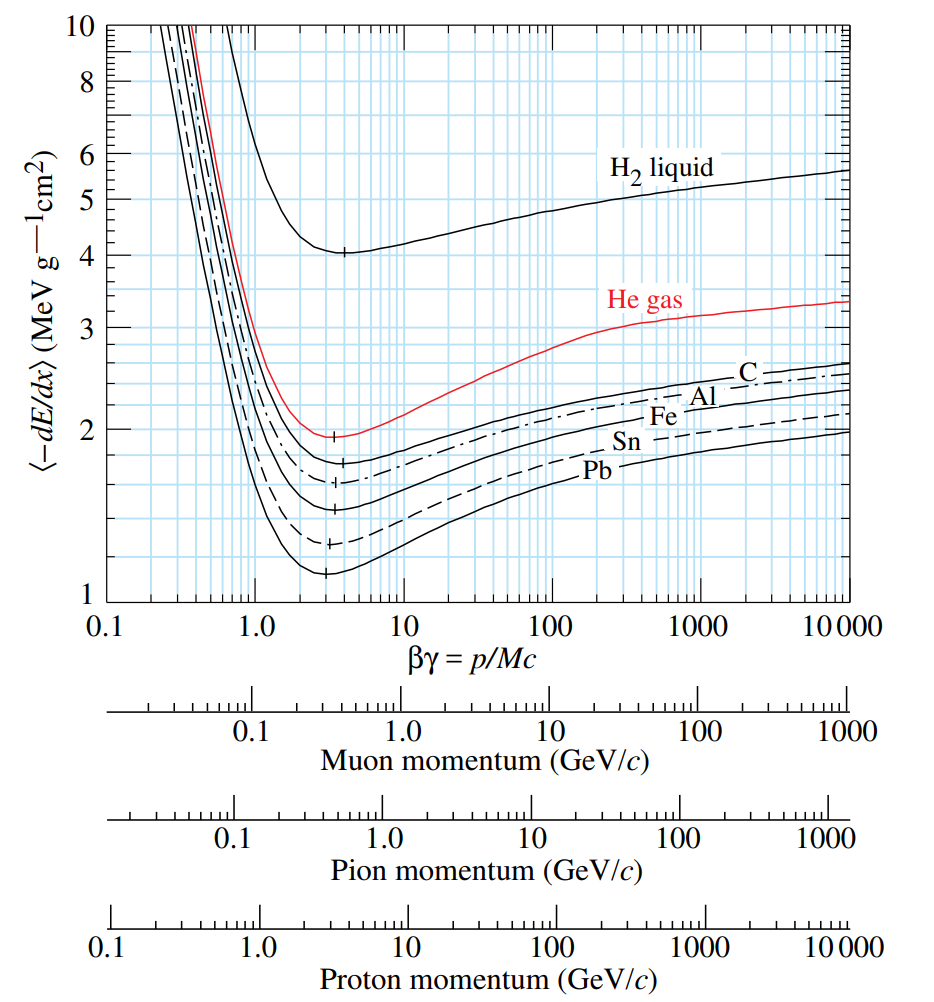
\includegraphics[width=10cm]{immagini/grafico_bethe_bloch.png}
\end{figure}
In ascisse è riportato il valore $\beta\gamma=p/Mc$ della particella incidente, ovvero l'impulso scalato rispetto alla massa, in modo da rendendoci indipendenti da quest'ultima. Ovviamente potremmo riportare semplicemente l'impulso, ma ciò significherebbe che i valori delle ascisse differirebbero in base al tipo di particella (come possiamo vedere in figura); sulle ordinate è riportata la perdita di energia in unità di densità superficiale. Per entrambi gli assi la scala è logaritmica; inoltre le varie curve sono relative a diversi materiali attraversati.

Consideriamo ad esempio un protone che incide su piombo Pb. La perdita di energia dipenderà dall'impulso del protone: per impulsi bassi la perdita di energia ha valori elevati, intorno a $10 \; \rm MeV \, cm^2/g$, man mano che consideriamo protoni con impulso maggiore la perdita di energia diventa sempre più bassa, fino a raggiungere un valore minimo leggermente maggiore di $1 \; \rm MeV \, cm^2/g$. Una volta superato il minimo abbiamo una risalita, dovuta alla risalita relativistica della formula di Bethe-Bloch. Se allora dobbiamo individuare quali sono le zone del grafico influenzate dai diversi fattori della 
formula, possiamo dire che

\begin{itemize}
    \item la regione a sinistra del minimo è influenzata dall'andamento grosso modo iperbolico di $1/\beta^2$ ;
    \item la regione a destra del minimo è influenzata dalla risalita relativistica, che ha un andamento logaritmico di $E$.
\end{itemize}

\begin{minipage}{0.465\textwidth}
    \begin{figure}[H]
        \centering
        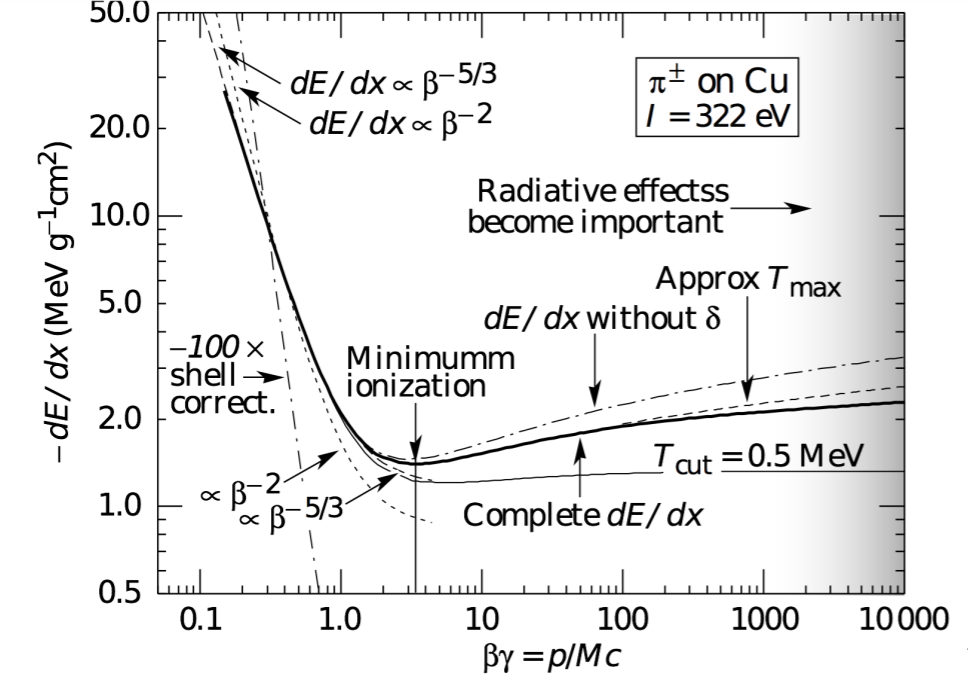
\includegraphics[width=7cm]{immagini/correzioni_shell_densita.png}
    \end{figure}
\end{minipage}
\begin{minipage}{0.53\textwidth}
    \vspace{0.4cm}Ricordiamo inoltre che nella regione all'estrema sinistra ad impulsi più bassi interviene il fattore correttivo di shell, mentre quella all'estrema destra ad impulsi più alti è influenzata dal fattore correttivo di densità.

    In figura possiamo vedere il grafico relativo a pioni che incidono su rame Cu. Le linee tratteggiate mostrano come sarebbe il grafico se non considerassimo i fattori correttivi.
\end{minipage}

\subsection{Perdita di energia per composti}

Consideriamo il caso in cui il materiale su cui incide la particella non è formato da un solo elemento bensì è un composto, cioè è costituito da atomi di diversi elementi. In tal caso, per calcolare la perdita di energia si fa una sorta di media pesata, data da

\begin{equation*}
    \frac{1}{\rho} \dv{E}{x}
    =\sum_i \frac{n_i A_i}{\rho_i A} \qty( \dv{E}{x} )_i
\end{equation*}

dove $n_i$, $A_i$, $\rho_i$ e $(\dv*{E}{x})_i$ sono rispettivamente il numero di atomi, il peso atomico, la densità e la perdita di energia specifica della specie $i$-esima del composto.

Consideriamo ad esempio la molecola $\rm CH_2$: per essa abbiamo che
\begin{eqnarray*}
    n_{\rm C}=1 & A_{\rm C}=12\\
    n_{\rm H}=1 & A_{\rm H}=1
\end{eqnarray*}
quindi la perdita di energia sarà data da
\begin{equation*}
    \frac{1}{\rho} \dv{E}{x}
    =\frac{2 \cdot 12}{\rho_{\rm C} A} \qty( \dv{E}{x} )_{\rm C} + \frac{1 \cdot 1}{\rho_{\rm H} A} \qty( \dv{E}{x} )_{\rm H}
\end{equation*}

\subsection{Picco di Bragg}

Finora abbiamo parlato di stime medie della perdita di energia, ma abbiamo accennato al fatto che potrebbero esserci delle fluttuazioni rispetto a tale valore medio. Concentriamoci adesso su questo aspetto.

Consideriamo il seguente grafico, chiamato picco di Bragg:

\begin{minipage}{0.465\textwidth}
    \begin{figure}[H]
        \centering
        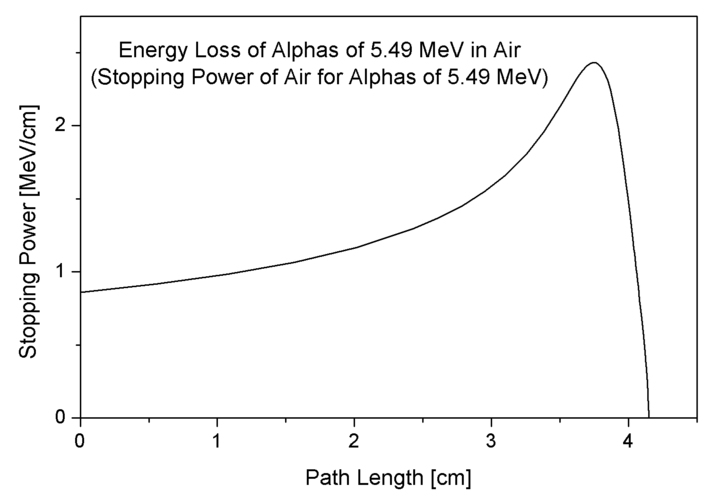
\includegraphics[width=7cm]{immagini/picco_di_Bragg.png}
    \end{figure}
\end{minipage}
\begin{minipage}{0.53\textwidth}
    In tale grafico la perdita di energia specifica è rappresentata in funzione dello spessore attraversato. In particolare il grafico mostrato è ottenuto da particelle $\alpha$ che attraversano l'aria, avendo un'energia di 5.49 MeV.
    
    La perdita di energia si calcolerà tramite Bethe-Bloch, in cui i valori di $\beta$ e $\gamma$ si ricavano da questo valore di energia iniziale.
\end{minipage}

\vspace{0.4cm}Man mano che la particella attraversa il materiale avvengono multiple collisioni con gli elettroni atomici e l'energia diminuisce. Di conseguenza $\dv*{E}{x}$ aumenta\footnote{Si può intuire che sia così leggendo da destra verso sinistra il grafico avente in ascisse l'impulso: man mano che la velocità diminuisce arriviamo nella regione in cui l'andamento è iperbolico, per cui la perdita di energia aumenta bruscamente. Un'altra maniera di visualizzare il fenomeno è che la particella, essendo più lenta, interagirà maggiormente con la materia.}, come osserviamo anche nel grafico, fino a raggiungere un valore massimo per poi diminuire bruscamente. Attenzione! Questa rapida discesa non è evidenziata nei precedenti grafici, in cui manca una parte ad energie ancora più basse, dove intervengono diversi fattori che fanno sì che la curva torni a zero. La parte finale del picco di Bragg è quindi dovuta al fatto che la particella si sta arrestando, avendo velocità e impulsi quasi nulli, per cui la perdita di energia va a zero\footnote{Come riportato dal Knoll, "[...] la formula di Bethe-Bloch inizia ad essere fallace ad energie basse, dove lo scambio di carica tra particella e assorbitore diventa rilevante. La particella carica positivamente tenderà a strappare elettroni dall'assorbitore, riducendo così la sua carica e di conseguenza il $\dv*{E}{x}$. Alla fine della sua traiettoria, la particella avrà accumulato $z$ elettroni diventando così un atomo neutro.".}. Da ciò capiamo che tale grafico è una diretta conseguenza del grafico visto precedentemente.

Il picco di Bragg è alla base dell'utilizzo delle radiazioni per la cura dei tumori, perché ci dice che ad esempio un protone che attraversa un determinato spessore di materiale non rilascia la sua energia in maniera costante lungo il percorso, bensì deposita la maggior parte della sua energia in corrispondenza del picco, poco prima di arrestarsi. Ciò costituisce un vantaggio perché può essere usato per fare un rilascio mirato di energia in alcune zone del corpo. Il limite di questa tecnica sta nella profondità che si può raggiungere, perché per arrivare più in profondità serve maggiore energia e quindi acceleratori più potenti, che non sempre sono disponibili; inoltre quando si raggiungono energie molto elevate si possono indurre altri fenomeni di origine nucleare con produzione di altre particelle con il conseguente rischio di arrecare dei danni.

\section{Fluttuazioni statistiche nella perdita di energia}

Analizziamo ora le fluttuazioni statistiche.

Se inviamo sul materiale particelle identiche (stessa massa, stessa energia e stesso angolo di incidenza quindi stessa direzione di incidenza), esse non perderanno la stessa energia, in quanto ogni particella seguirà un percorso diverso, subendo un numero di collisioni diverso e perdendo di conseguenza un'energia diversa.

Le fluttuazioni statistiche che si presentano nella perdita di energia possono avere distribuzioni diverse, in particolare due:

\begin{minipage}{0.495\textwidth}
    \begin{figure}[H]
        \centering
        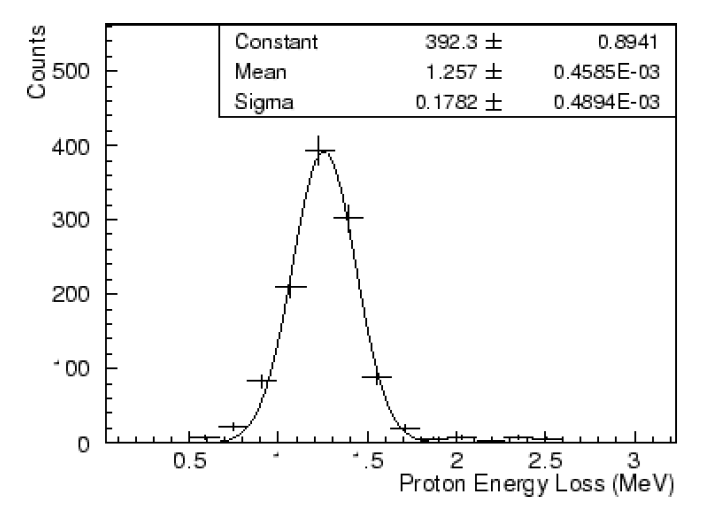
\includegraphics[width=6.5cm]{immagini/energy_loss_distribuzione_gauss.png}
        %\caption*{Distribuzione gaussiana.}
    \end{figure}

    \vspace{-0.8cm}

    \begin{figure}[H]
        \centering
        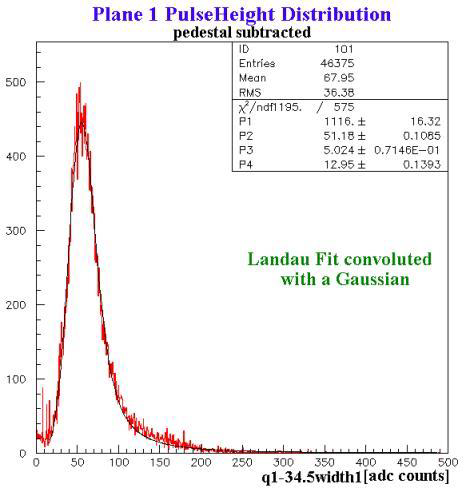
\includegraphics[width=6cm]{immagini/energy_loss_distribuzione_vavilov.png}
        %\caption*{Distribuzione di Landau-Vavilov.}
    \end{figure}
\end{minipage}
\begin{minipage}{0.5\textwidth}
    \vspace{1cm}Se consideriamo spessore grandi, ci si aspetta che il numero di collisioni sia elevato. Ciò fa sì che la distribuzione della perdita di energia in uno spessore grande abbia un andamento abbastanza simmetrico che segue la distribuzione di Gauss;
    
    \vspace{1.7cm}Se invece consideriamo spessori piccoli, il numero di collisioni è minore, e la perdita di energia segue una distribuzione che può essere descritta dalla teoria di Landau-Vavilov. È una distribuzione asimmetrica che presenta un picco e poi una lunga coda a valore elevati. Essa ci dice che, quando una particella attraversa uno spessore sottile, in media perde un certo quantitativo di energia, ma ci sono dei casi in cui può perdere anche valori notevoli di energia, magari perché la particella segue altre percorsi.
\end{minipage}

\vspace{0.4cm}Per valutare se uno spessore è grande o piccolo esiste un parametro che dipende dal valore dell'energia massima che si può perdere per singolo urto, il quale ci permette di individuare il regime in cui ci troviamo.

\comment{
\begin{approfondimento}[The Energy Loss Distribution]
    \footnotesize
    Quanto segue è tratto da \textit{William R. Leo - "Techniques for Nuclear and Particle Physics Experiments"}, section 2.6.
    
    \vspace{0.2cm}Finora la nostra discussione sulla perdita di energia si è concentrata principalmente sulla perdita di energia media che subiscono particelle cariche attraverso spessori di materiale. Tuttavia, per ogni particella la quantità di energia persa non sarà in generale uguale a tale valore medio a causa delle fluttuazioni statistiche che si verificano nel numero di collisioni che avvengono e nell'energia trasferita in ognuna di queste. Ne segue che un fascio inizialmente monoenergetico, dopo aver attraversato un determinato spessore di materiale, mostrerà una distribuzione in energia piuttosto che una delta di Dirac shiftata a sinistra di una quantità pari alla perdità media di energia così come dato dalla formula del $\dv*{E}{x}$.
    
    Da un punto di vista teorico, calcolare la distribuzione della perdita di energia per un dato spessore di materiale è un problema difficile dal punto di vista matematico ed è in generale diviso in due casi: assorbitori spessi e assorbitori sottili.
    
    \vspace{0.2cm}\textbf{Assorbitori spessi: il limite Gaussiano}
    
    Per assorbitori abbastanza spessi tali che il numero di collisioni sia grande, si può facilmente mostrare che la distribuzione della perdita di energia ha la forma di una Gaussiana. Ciò segue dal teorema del limite centrale in statistica, il quale afferma che la somma di $N$ variabili casuali che seguono tutte la stessa distribuzione statistica, tende a quella di una variabile che segue la distribuzione gaussiana nel limite $N \to +\infty$.
    
    Se come variabile casuale prendiamo l'energia persa in una singola collisione atomica $\dd{E}$ e assumiamo che questa sia tale che la variazione della velocità della particella sia trascurabile (così che la dipendenza dalla velocità della sezione d'urto resti costante), allora l'energia persa in totale è pari alla somma di diversi $\dd{E}$ indipendenti, tutti distribuiti uniformemente. Assumendo che ci sia un numero sufficiente di collisioni $N$, allora il totale tenderà alla forma gaussiana,
    \begin{equation*}
        f(x,\Delta) \propto \exp{ - \frac{\qty(\Delta - \bar{\Delta})^2}{2\sigma^2} }
    \end{equation*}
    
    dove $x$ è lo spessore dell'assorbitore, $\Delta$ la perdita di energia nell'assorbitore, $\bar{\Delta}$ la perdita di energia media e $\sigma$ la deviazione standard.

    \comment{Per particelle pesanti non relativistiche la larghezza $\sigma_0$ di questa Gaussiana fu calcolata da Bohr, che ottene come valore
        \begin{equation*}
            \sigma_0^2
            =4\pi N_a r_e^2 \qty(m_e c^2)^2 \rho \frac{Z}{A} x
            =0.1569 \frac{Z}{A} x
        \end{equation*}
    where $N_a$ è il numero di Avogadro, $r_e$ e $m_e$ il raggio e la massa classica dell'elettrone e $\rho$, $Z$ e $A$ sono rispettivamente la densità, il numero atomico e  and
    p, Z, A are the density, atomic number and atomic weight of the material respectively.
    This formula can easily be extended to relativistic particles
    \begin{equation*}
        \sigma^2=\frac{\qty( 1 - \frac{1}{2}\beta^2 )}{1 - \beta^2}\sigma_0^2
    \end{equation*}
    }
        \begin{equation*}
            \kappa=\frac{\bar{\Delta}}{W_{\rm max}}
        \end{equation*}
        \begin{equation*}
            \bar{\Delta} \simeq \xi
            =2\pi N_a r_e^2 m_e c^2 \rho \frac{Z}{A} \qty( \frac{z}{\beta} )^2 x
        \end{equation*}
        \textbf{Assorbitori sottili}

        A differenza del caso precedente, la distribuzione per assorbitori sottili, in cui il numero di collisioni è troppo piccolo per poter valere il teorema del del limite centrale, è estremamente complicata da valutare. Ciò è dovuto alla possibilità di grandi trasferimenti di energia in una singola collisione. Per particelle pesanti, questa $W_{\rm max}$ è approssimabile all'espressione
        \begin{equation*}
            W_{\rm max} \simeq 2 m_e c^2 (\beta\gamma)^2
        \end{equation*}
        In contrast to the thick absorber case, the distribution for thin absorbers or gases where
the number of collisions N is too small for the Central Limit Theorem to hold is extremely
complicated to calculate. This is because of the possibility of large energy
transfers in a single collision. For heavy particles, this W max is kinematically limited to
the expression given in (2.28), while for electrons, as much as one-half the initial energy
can be transferred. In this latter case, there is also the additional possibility of a large
"one-shot" energy loss from bremsstrahlung as well. While these events are rare, their
possibility adds a long tail to the high energy side of the energy-loss probability distribution
thus giving it a skewed, asymmetric form. Figure 2.18 illustrates this general
shape. Note that the mean energy loss no longer corresponds to the peak but is displaced
because of the high energy tail. In contrast, the position of the peak now defines
the most probable energy loss. These two quantities may be used to parametrize the
distribution.
£
:0
d
.Q
o
0.
Most Energy loss L1
probable Mean
energy energy
loss loss
Fig. 2.18. Typical distribution of energy loss in a
thin absorber. Note that it is asymmetric with a long
high energy tail
Basic theoretical calculations of this distribution have been carried out by Landau,
Symon and Vavilov; each of these, however, has a somewhat different region of applicability.
The distinguishing parameter in all these theories is the ratio
(2.96)
that is the the ratio between the mean energy loss and the maximum energy transfer allowable
in a single collision. The mean energy loss may be calculated from the BetheBloch
formula, however, for most purposes it is usually approximated by taking the
first multiplicative term only and ignoring the logarithmic term, i.e.,
        Following the literature, we denote this quantity by ~. The thin absorber region is
generally taken to be K < 10, although for K> 1, the distribution already begins to approach
the the Gaussian limit (see Fig. 2.19). By K>10, there, of course, is only a very
negligible difference.
    \end{approfondimento}
    
    } %fine commento

\subsection{Range di una particella}

Come abbiamo appena detto, anche se le condizioni sono uguali (stessa tipo di particella incidente, stessa energia ecc.), l'energia persa non è sempre la stessa. Ciò deriva dai processi di fluttuazioni statistiche dovuti alle diverse collisioni che una particella può subire all'interno del materiale: essendo le collisioni parecchie, ogni particella avrà un suo percorso e dunque una sua perdita di energia. Vediamo che effetto hanno tali fluttuazioni sul range di una particella.

Per range di una particella si intende il percorso effettuato da questa all'interno di un mezzo prima di arrestarsi.

Prima di andare a fare un confronto tra cosa ci aspetteremmo idealmente e cosa realmente osserviamo, dobbiamo definire il \textit{coefficiente di trasmissione}. Per capire cos'è quest'ultimo immaginiamo di inviare delle particelle con una data energia iniziale $E$ su uno spessore di materiale $\Delta x$. Immaginiamo poi che il flusso di particelle incidenti (che si misura in particelle per unità di superficie al secondo) sia pari ad un valore $I_0$.

\begin{minipage}{0.295\textwidth}
    \begin{figure}[H]
        \centering
        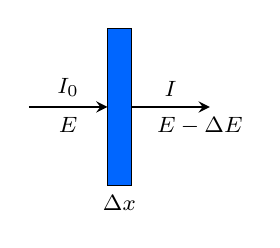
\begin{tikzpicture}
            \draw[fill=blue!60!cyan!] (0,-1) rectangle (+0.3cm,+1cm);
            \node[below] at (0.15,-1) {\footnotesize$\Delta x$};
            \draw[thick, -stealth] (-1,0) -- (0,0) node [midway, above] {\footnotesize$I_0$} node [midway, below] {\footnotesize$E$};
            \draw[thick, -stealth] (0.3,0) -- (1.3,0) node [midway, above] {\footnotesize$I$} node [below right] {\footnotesize\hspace{-0.8cm}$E - \Delta E$};
        \end{tikzpicture}
    \end{figure}
\end{minipage}
\begin{minipage}{0.7\textwidth}
    \vspace{0.2cm}Supponiamo di misurare un flusso in uscita pari $I$, che corrisponde a quante particelle sopravvivono all'attraversamento del materiale. In base allo spessore verrà persa una certa quantità di energia $\Delta E$, per cui le particelle che riescono a fuoriuscire avranno energia $E - \Delta E$.
\end{minipage}

\vspace{0.2cm}Numericamente il $\Delta E$ può essere valutato mediante la relazione

\begin{equation*}
    \Delta E=\expval{\dv{E}{x}}\Delta x
\end{equation*}

Tuttavia in questo mondo stiamo compiendo un'inesattezza: stiamo supponendo che il $\dv*{E}{x}$ sia costante, ma esso è funzione dell'energia, per cui come vedremo il modo corretto per valutarlo è mediante un integrale.

Sotto l'ipotesi di $\dv*{E}{x}=\rm cost.$, ci aspettiamo che all'aumentare di $\Delta x$ aumenti anche $\Delta E$. Se non ci fossero fluttuazioni statistiche, ci aspetteremo che finché $\Delta x$ è piccolo le particelle perdono una certa energia $\Delta E$ ma riescono comunque a passare, per cui si avrebbe che $I=I_0$, cioè si misura un numero di particelle per unità di tempo e superficie in uscita pari a quelle in entrata; man mano che si aumenta $\Delta x$ si arriverebbe ad un punto in corrispondenza del quale la perdita di energia $\Delta E$ coinciderà con l'energia totale $E$ della particella, che quindi viene persa completamente. Pertanto, superato questo spessore, ci aspetteremmo che nessuna particella dovrebbe riuscire ad attraversare lo spessore. Allora il coefficiente di trasmissione $T$, definito come

\begin{equation*}
    T=\frac{I}{I_0}
    \qquad
    \qty[ \frac{\text{n° particelle uscenti}}{\text{n° particelle incidenti}} ]
\end{equation*}

al variare di $\Delta x$ dovrebbe avere un andamento piatto pari a 1 fino ad un certo valore $R$, raggiunto il quale diventa nullo in quanto in tale punto la perdita di energia diventa pari proprio a $E$.\footnote{In altre parole, nel caso ideale in assenza di fluttuazioni statistiche (il che significherebbe che le particelle seguirebbero tutte lo stesso percorso, subendo un uguale numero di collisioni e quindi perdendo la stessa energia), ci aspettiamo un andamento a gradino.} Lo spessore $R$ prende il nome di range della particella perché è proprio lo spessore attraversato dalla particella finché non si arresta.

Nella realtà intervengono le fluttuazioni statistiche, che rendono il percorso di ciascuna particella peculiare. Ne segue che di volta in volta si può perdere più o meno energia e di conseguenza la particella si fermerà rispettivamente prima o dopo rispetto a $R$. Ciò fa sì che la curva ottenuta è una sorta di sigmoide, che parte da 1 ma poi si smussa, per cui non c'è un passaggio netto dalla situazione in cui la particella passa a quella in cui non passa. Questa è la curva che osserviamo sperimentalmente\footnote{Per misurare sperimentalmente il range di una particella dovremmo avere una sorgente che emette la particelle a una data energia, un rivelatore posizionato a una certa distanza e a quel punto effettuiamo delle misure interponendo spessori di un dato materiale via via crescenti, andando a misurare il numero di particelle osservate rispetto al numero di particelle senza nessuno spessore.}.

\begin{minipage}{0.5\textwidth}
    \begin{figure}[H]
      \centering
      \begin{tikzpicture}[scale=.6]
        \draw[->] (0,0) -- (0,5) node[above] {$T$};
        \draw[->] (0,0) -- (5.5,0) node[right] {$\Delta x$};
        \draw[thick,red] (0,4) node[black,left] {$1$} -- (3,4) -- (3,0) -- (5,0);
        \node[below] at (3,0) {$R$};
      \end{tikzpicture}
      \caption*{Caso ideale.}
    \end{figure}
  \end{minipage}
  \begin{minipage}{0.5\textwidth}
    \begin{figure}[H]
      \centering
      \begin{tikzpicture}[scale=.6]
        \draw[->] (0,0) -- (0,5) node[above] {$T$};
        \draw[->] (0,0) -- (5.5,0) node[right] {$\Delta x$};
        \draw[dashed] (3,2) -- (3,0) node[below] {$R$};
        \draw[thick,teal!60!green] (0,4) node[black,left] {$1$} -- (1,4) -- plot[smooth,domain=-2:2] (3+\x, {4*(1-exp(4.5*\x)/(1 + exp(4.5*\x)))});
      \end{tikzpicture}
      \caption*{Caso reale.}
    \end{figure}
\end{minipage}

\vspace{0.3cm}Il grafico così realizzato prende il nome di \textit{grafico di trasmissione}. Sulle ascisse riportiamo lo spessore attraversato, che può essere espresso sia in unità lineari (ad esempio cm) che in unità superficiali, mentre in ordinate il coefficiente di trasmissione. Esso si può definire per qualsiasi radiazione e può essere utile per determinare che spessore di materiale adoperare per essere schermati da un tipo di radiazione.

Analizziamo adesso in maniera più dettagliata la curva di trasmissione:

\vspace{-0.3cm}

\begin{figure}[H]
    \centering
    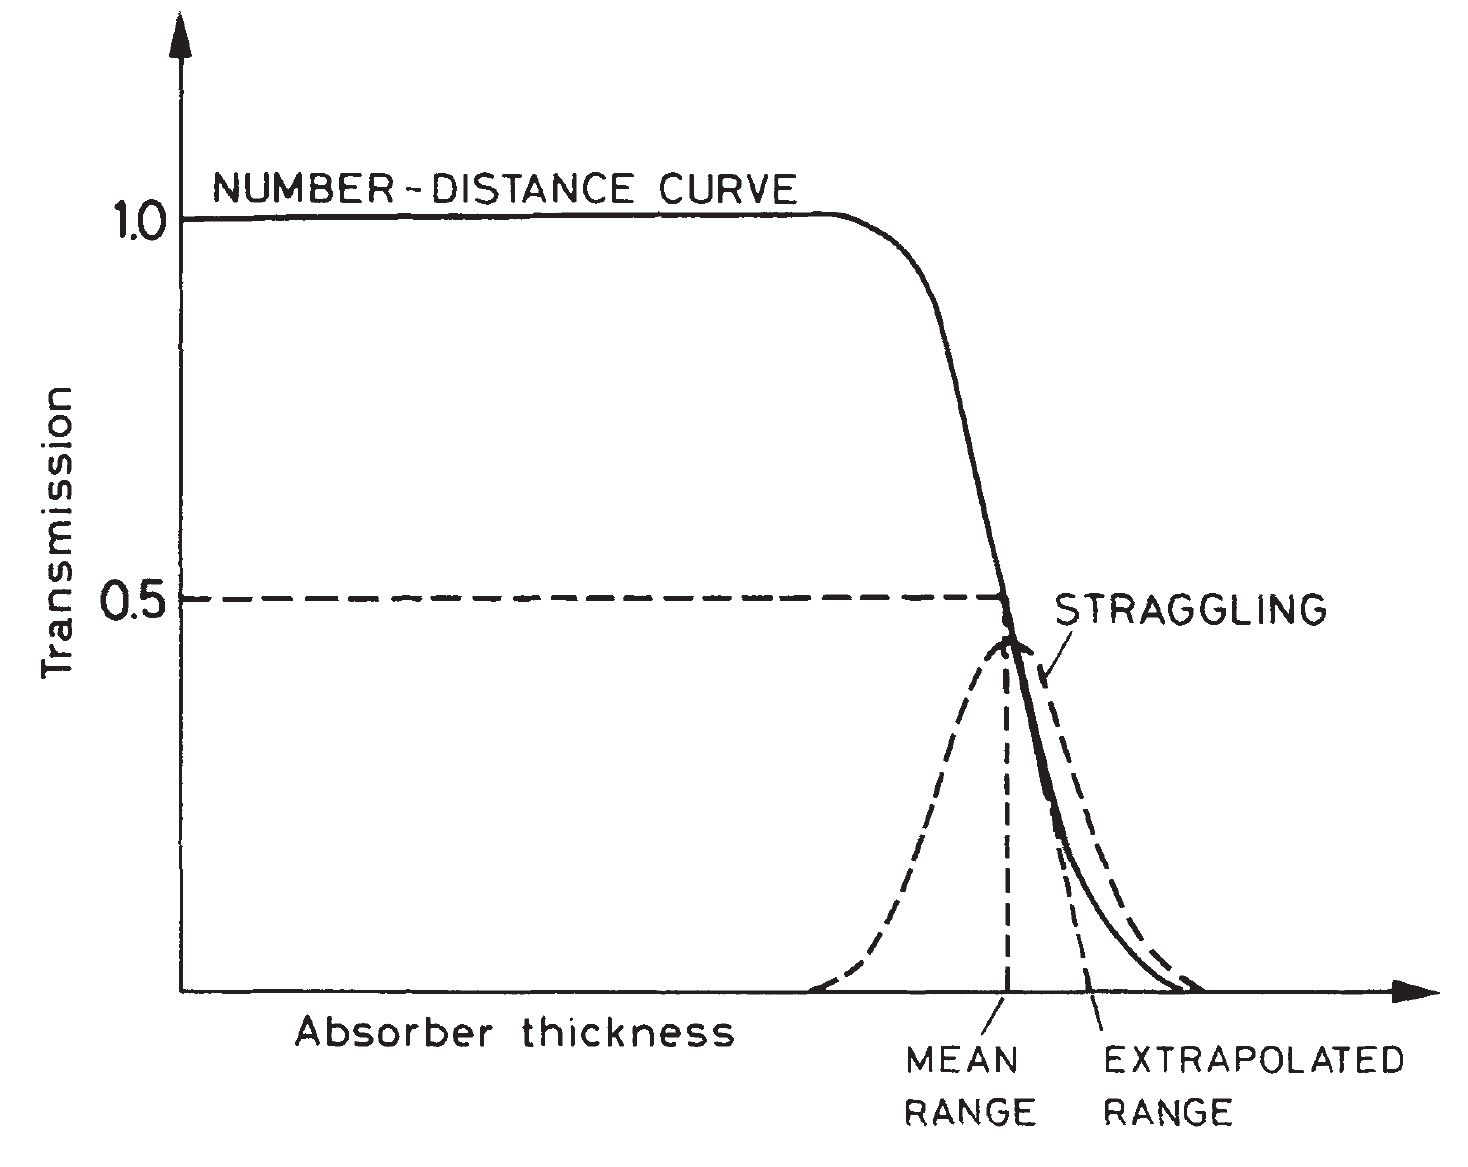
\includegraphics[width=8cm]{immagini/straggling.png}
\end{figure}

\vspace{-0.4cm}

La dispersione dell'energia depositata e del range della particella prendono il nome di \textit{effetti di straggling}, cioè di allargamento: mentre idealmente $R$ è un valore definito, nei fatti è difficile da definire in quanto ogni particella ha un suo range, nel senso che si può fermare prima o dopo rispetto al valore nominale. \E comunque possibile definire il range di una particella: dal grafico possiamo ricavare il range medio, spessore in corrispondenza del quale il fascio viene dimezzato (cioè riescono a passare solo il 50\% delle particelle). In alternativa, si può ricavare il range estrapolato, definito come l'intersezione della tangente alla sigmoide nel punto del range medio con l'asse delle ascisse.

Nel grafico figura anche una gaussiana: essa rappresenta lo spessore percorso da un certo numero di particelle prima di fermarsi, che non sempre è lo stesso, per cui abbiamo una distribuzione di valori centrata intorno al valor medio e con una certa larghezza che dipende dalle caratteristiche della particella e del materiale.

\E chiaro che maggiori sono le fluttuazioni nel range, più la sigmoide sarà smussata, se invece le fluttuazioni sono piccole la curva tenderà sempre più ad una curva a gradino. Nel caso particolare di particelle cariche pesanti la sigmoide è molto vicina ad una curva a gradino.

Oltre che per la funzione di schermaggio, il range può essere usato per valutare lo spessore che deve avere un rivelatore per arrestare totalmente una particella e quindi misurarne tutta l'energia.

Oltre che in termini di range, gli effetti di straggling si manifestano anche in termini energetici.

\begin{figure}[H]
    \centering
    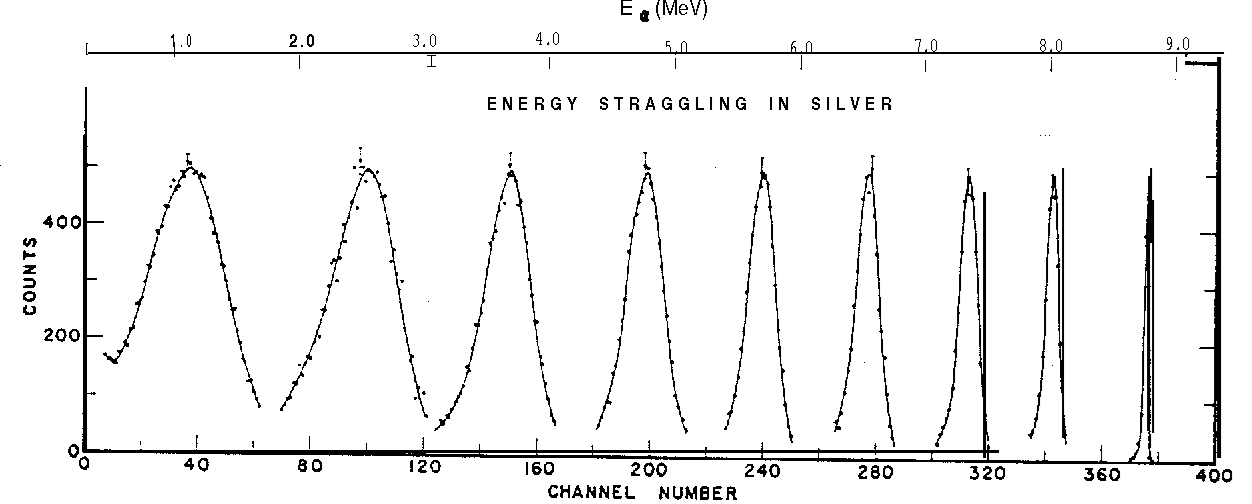
\includegraphics[width=12cm]{immagini/straggling_energie.png}
\end{figure}

Nel grafico possiamo vedere degli spettri di energia ottenuti da un rivelatore che misura l'energia di particelle provenienti da una sorgente ad energia fissata $E$ al variare dello spessore di materiale assorbitore interposto.

Senza interporre alcun materiale tra sorgente e rivelatore, quello che si dovrebbe misurare dovrebbe essere una delta di Dirac, cioè idealmente dovremmo misurare sempre lo stesso valore di energia con cui vengono emesse dalla sorgente, ed è ciò che si osserva nel picco più a destra, il quale ha una sua larghezza per motivi di risoluzione dell'apparato sperimentale. Il fatto che sia un picco molto stretto ci dice che l'energia delle particelle che stanno arrivando assume quasi sempre lo stesso valore, con delle fluttuazioni molto piccole.

Se adesso interpretiamo un materiale tra sorgente e rivelatore, le particelle incideranno su di esso, e se questo è sufficientemente sottile riusciranno ad attraversarlo perdendo una parte della loro energia, per cui giungeranno al rivelatore con un'energia degradata pari a $E - \Delta E$; ne segue che andando a misurare l'energia delle particelle adesso vedremo il picco spostato a sinistra, a valori un po' più piccoli; inoltre esso si allarga. Questo effetto di allargamento diventa sempre più evidente man mano che aumenta lo spessore, infatti i picchi che vediamo in figura andando verso sinistra sono stati ottenuti interponendo spessori via via crescenti. \E chiaro che se stiamo misurando qualcosa significa che gli spessori sono inferiori al range della particella, altrimenti non misureremo nulla perché le particelle verrebbero arrestate.

Il fatto che le distribuzioni si allargano ci dice che è come se ci fosse una indeterminazione maggiore nell'energia residua della particella, che equivale a delle fluttuazioni nell'energia depositata nel materiale, che sono tanto più grandi quanto maggiore è lo spessore di materiale interposto. 

In sintesi, un altro modo di mettere in evidenza gli effetti di straggling è quello di interporre materiale con spessore via via maggiore: quello che si osserva è non solo una maggiore perdita di energia, ma anche che quest'ultima ha delle fluttuazioni via via più geandi.

%vengono evidenziati sempre più man mano che aumentiamo lo spessore del materiale interposto si evidenziano come maggiori fluttuazioni nella perdita di energia.

\subsection{Il channeling}

Per quanto riguarda la perdita di energia per collisioni, si deve fare un discorso leggermente diverso quando si parla di materiali cristallini.

\begin{minipage}{0.395\textwidth}
    \begin{figure}[H]
        \centering
        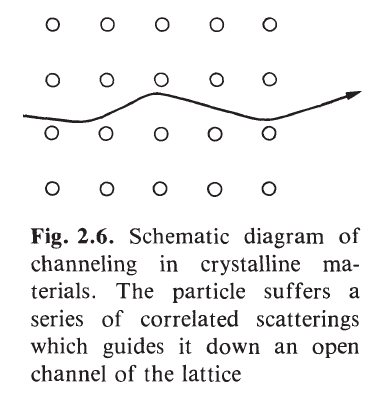
\includegraphics[width=6cm]{immagini/channeling.png}
    \end{figure}
\end{minipage}
\begin{minipage}{0.6\textwidth}
    \vspace{0.4cm}In questi infatti si può verificare un altro effetto che prende il nome di channeling, cioè la particella, entrando con un opportuno angolo di incidenza, potrebbe seguire un percorso tra i piani del cristallo, quindi subirà meno collisioni di quante ne avrebbe avute con un angolo di incidenza diverso o attraversando un materiale amorfo. Nei casi di channeling la formula di Bethe-Bloch sovrastima la perdita di energia, nel senso che nei fatti si perde meno energia del valore teorico in virtù del fatto che le particelle seguono un percorso particolare.
\end{minipage}

\vspace{0.2cm}Per verificarsi tale effetto il materiale deve essere cristallino, cioè dotato di una struttura ordinata di atomi e la particella deve entrare nel cristallo con un angolo di incidenza molto piccolo rispetto all'asse di simmetria del cristallo.

\subsection{Come calcolare il range di una particella}

Da un punto di vista teorico, il range medio di una particella che incide su un materiale con energia $E_{\rm inc}$ si può calcolare mediante l'integrale

\begin{equation*}
    R(E_{\rm inc})=\int_{0}^{E_{\rm inc}} \qty( \dv{E}{x} )^{-1} \dd{E}
\end{equation*}

il quale può essere valutato mediante integrazione numerica.

\section{Radiazione Cherenkov}

È uno dei possibili meccanismi di perdita di energia. L'emissione di tale radiazione avviene quando la velocità della particella nel mezzo supera la velocità della luce nello stesso mezzo. Quest'ultima è data da

\begin{equation*}
    \beta c=v=\frac{c}{n}
\end{equation*}

dove $n$ è l'indice di rifrazione del mezzo e $c$ la velocità della luce nel vuoto. Ne segue che la condizione affinché una particella emetta radiazione Cherenkov è

\begin{equation*}
    v_{\rm part} > \frac{c}{n}
\end{equation*}

\E un po' lo stesso effetto che avviene per il suono con il cosiddetto "cono di Mach", che si presenta quando si supera la velocità del suono in quel mezzo. In questo caso viene generata un'onda d'urto elettromagnetica con fronte d'onda conico.

\begin{minipage}{0.395\textwidth}
    \begin{figure}[H]
        \centering
        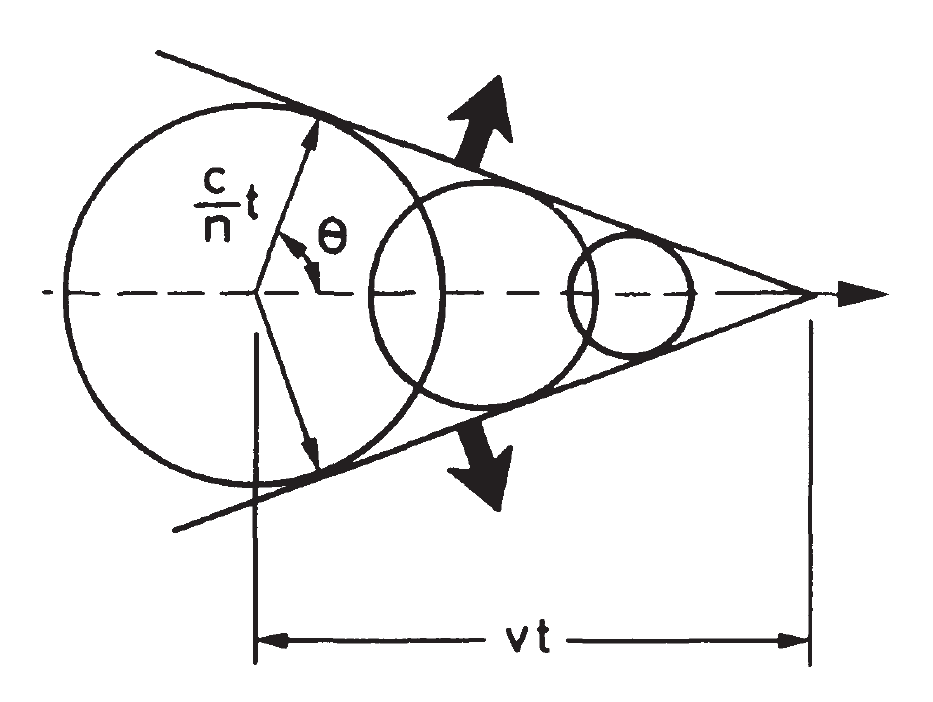
\includegraphics[width=5cm]{immagini/Effetto_Cherenkov.png}
    \end{figure}
\end{minipage}
\begin{minipage}{0.6\textwidth}
    \vspace{0.6cm}Tale radiazione è direzionata: viene messa all'interno di un cono con una certa apertura, la quale dipende da $n$ e dalla velocità della particella: maggiore è la velocità, minore sarà l'apertura del cono
    \begin{equation*}
        \vartheta_{\rm Ch}
        =\arccos{\left(\frac{1}{\beta n}\right)}
    \end{equation*}
\end{minipage}

\vspace{0.2cm}La radiazione emessa ha uno spettro continuo, nel senso che non ci sono dei valori di frequenza privilegiati; tuttavia, concentrandoci nel visibile, questo spettro è proporzionale alla frequenza, per cui si ha una maggiore emissione nel blu.

\E una luce polarizzata linearmente e la perdita di energia $\dv*{E}{x}$ dovuta a questo effetto (che è già inclusa nella formula di Bethe-Bloch, sebbene trascurabile) è un contributo piccolo, che vale $10^{-3}$ $\rm MeV \, cm^2/g$ per i solidi e $10^{-1}$-$10^{-2}$ $\rm MeV \, cm^2/g$ per i gas, mentre nei grafici precedenti il minimo di ionizzazione si trova a 1-2 $\rm MeV \, cm^2/g$. Tuttavia essa è da menzionare per l'uso che se ne fa in fisica. Ad esempio viene adoperata per rivelare particelle: un esempio si ha in astronomia, dove TeV di radiazioni gamma incidono sulla atmosfera, producendo coppie elettrone-positrone e queste particelle producono radiazione Cherenkov nell'atmosfera. Se abbiamo un rivelatore in grado di misurare tale radiazione (telescopio Cherenkov), possiamo andare effettuare misure dei gamma di partenza, ed essendo una luce direzionata possiamo anche ricostruire la direzione di arrivo dei gamma.

Un'applicazione simile si ha nella fisica dei neutrini, i quali interagiscono pochissimo con la materia, per cui per rivelarli sono necessari rivelatori di grandi volumi in modo da aumentare la probabilità di interazione. A causa di ciò, negli ultimi anni si è pensato che anziché usare oggetti creati dall'uomo si possono usare risorse naturali come l'acqua del mare e il ghiaccio, ponendo in essi dei rivelatori e usandoli come materiale attivo di rivelazione. L'idea è che ad esempio un neutrino attraversi km di acqua, interagisca e produca un muone, il quale produce effetto Cherenkov. Se siamo in grado di misurare tale luce, abbiamo indirettamente misurato l'arrivo di un neutrino. Ne è un esempio il Km3net: torri di rivelatori di luce (fotomoltiplicatori) calate in mare per andare a misurare la radiazione Cherenkov con lo scopo di misurare i neutrini.

Nel campo della fisica delle particelle e della fisica nucleare esistono i rivelatori Cherenkov, i quali servono a identificare le particelle, perché attraverso la rivelazione del cono Cherenkov cioè di questa luce abbiamo informazioni sulle particelle: dalla velocità possiamo ricavare l'impulso e quindi la massa, la quale ci permette di identificare le particelle. Esistono poi i contatori Cherenkov, che permettono di misurare particelle davanti velocità al di sopra di una certa soglia.

Tale radiazione viene usata nei reattori a fissione per andare a misurare l'attività presente, in quanto nei processi di fissione si generano sempre particelle cariche che producono radiazione Cherenkov.

\section{Possibili esercizi}

\begin{esercizio}
    Valutare la perdita di energia di particelle $\alpha$ da 5 Mev in un foglio di carta alluminio da cucina. Dati:

    \begin{itemize}
        \item Spessore fogli della carta da cucina: $0.016$ mm;
        \item Densità alluminio: $2.7 \; \rm g/cm^3$;
        \item Densità superficiale: $2.7 \cdot 0.0016 \rm \; g/cm^2=0.004 \; g/cm^2$.
    \end{itemize}
    
    Per tale attività serve la formula di Bethe-Bloch e poi bisogna costruire un grafico dei valori di perdita di energia specifica al variare dello spessore del foglio. La perdita di energia si calcolerà come
    \begin{equation*}
        \Delta E=\qty(\dv{E}{x}) \Delta x
    \end{equation*}
    con $\dv*{E}{x}$ calcolato con Bethe-Bloch.

    Attenzione! Questa formula è un'approssimazione: sarebbe valida se $\dv*{E}{x}$ fosse costante al variare di $x$. Nella realtà sappiamo che man mano che la particella penetra nel materiale perde energia e di conseguenza $\dv*{E}{x}$ cambia. Essa è comunque valida per valori piccoli di $\Delta x$.
\end{esercizio}

\begin{esercizio}
    Valutare la perdita di energia di muoni cosmici verticali (al minimo di ionizzazione) in
    \begin{enumerate}[label=\alph*.]
        \item una lastra di ferro di 10 cm di spessore;
        \item un solaio di cemento di 30 cm di spessore.
    \end{enumerate}
    Stavolta non viene fornito l'impulso della particella, viene detto che incidono verticalmente sulla lastra e si trovano al minimo di ionizzazione, pertanto dobbiamo ricavare graficamente tale valore. Un'altra difficoltà è il fatto che il cemento non è una sostanza pura, per cui dobbiamo capirne la composizione e fare una stima della perdita di energia usando la formula della perdita di energia per i composti.
    
    Da tale esperienza deduciamo che con tali spessori i muoni perdono energia ma riescono ad attraversare il materiale.
\end{esercizio}

\begin{esercizio}
    Valutare lo spessore necessario per degradare in energia un fascio di protoni da 600 MeV fino a portarli a 500 MeV mediante uno spessore di Rame (vedi Esempio 2.2 nel Leo).
\end{esercizio}

\subsection*{Il potenziale di ionizzazione medio}

Alcuni termini della formula di Bethe-Bloch possono essere definiti in diverso modo. Ne è un esempio il potenziale di ionizzazione medio, che abbiamo indicato con $I$ e può essere definito come:

\begin{itemize}
    \item Un valore proporzionale a $Z$;
    \item Un valore costante valido per tutti gli atomi, sebbene in realtà esso vari in base al numero atomico: varia molto negli elementi leggeri, per poi stabilizzarsi per elementi pesanti. Si può allora pensare di farne un valor medio;
    \item Una formula per parametrizzare se siamo in regime di nuclei leggeri o pesanti;
    \item Un valore preso da tabelle.
\end{itemize}

\subsection*{Come tenere conto di uno spessore finito}

Per valutare la perdita di energia in uno spessore finito inizialmente abbiamo usato l'approssimazione con cui valutavamo il $\dv*{E}{x}$ in corrispondenza dell'energia incidente iniziale e moltiplicavamo questo per lo spessore attraversato $\Delta x$. Ciò che in realtà è corretto fare è dividere il $\Delta x$ in tanti piccoli spessori $\dd{x}$, valutare lo stopping power all'inizio di ciascun intervallino, cioè cerchiamo di capire quant'è l'energia in ingresso, calcoliamo il $\dv*{E}{x}$ e poi la perdita di energia in tale spessore. Dopodiché passiamo allo spessore successivo in cui le energie in ingresso sarà data alla differenza dell'energia di prima meno la perdita di energia $\dd{E}$. Si procede per passi di $\dd{x}$ fin quando valutiamo la perdita di energia complessiva in tutto lo spessore. Con tale metodo teniamo conto del fatto che la perdita di energia assume via via un valore diverso, la quale aumenta man mano che la particella penetra nel materiale.